\documentclass{article}

\usepackage{graphicx}
\usepackage{tikz}
\usepackage{tikzsymbols}
\usetikzlibrary{calc,patterns,shapes.geometric}
\pagestyle{empty}
\usepackage[margin=0pt]{geometry}
\geometry{papersize={14in,12in}}

\def\centerarc[#1](#2)(#3:#4:#5){\draw[#1] ($(#2)+({#5*cos(#3)},{#5*sin(#3)})$) arc (#3:#4:#5);}

\begin{document}
	\begin{figure}
		\centering
		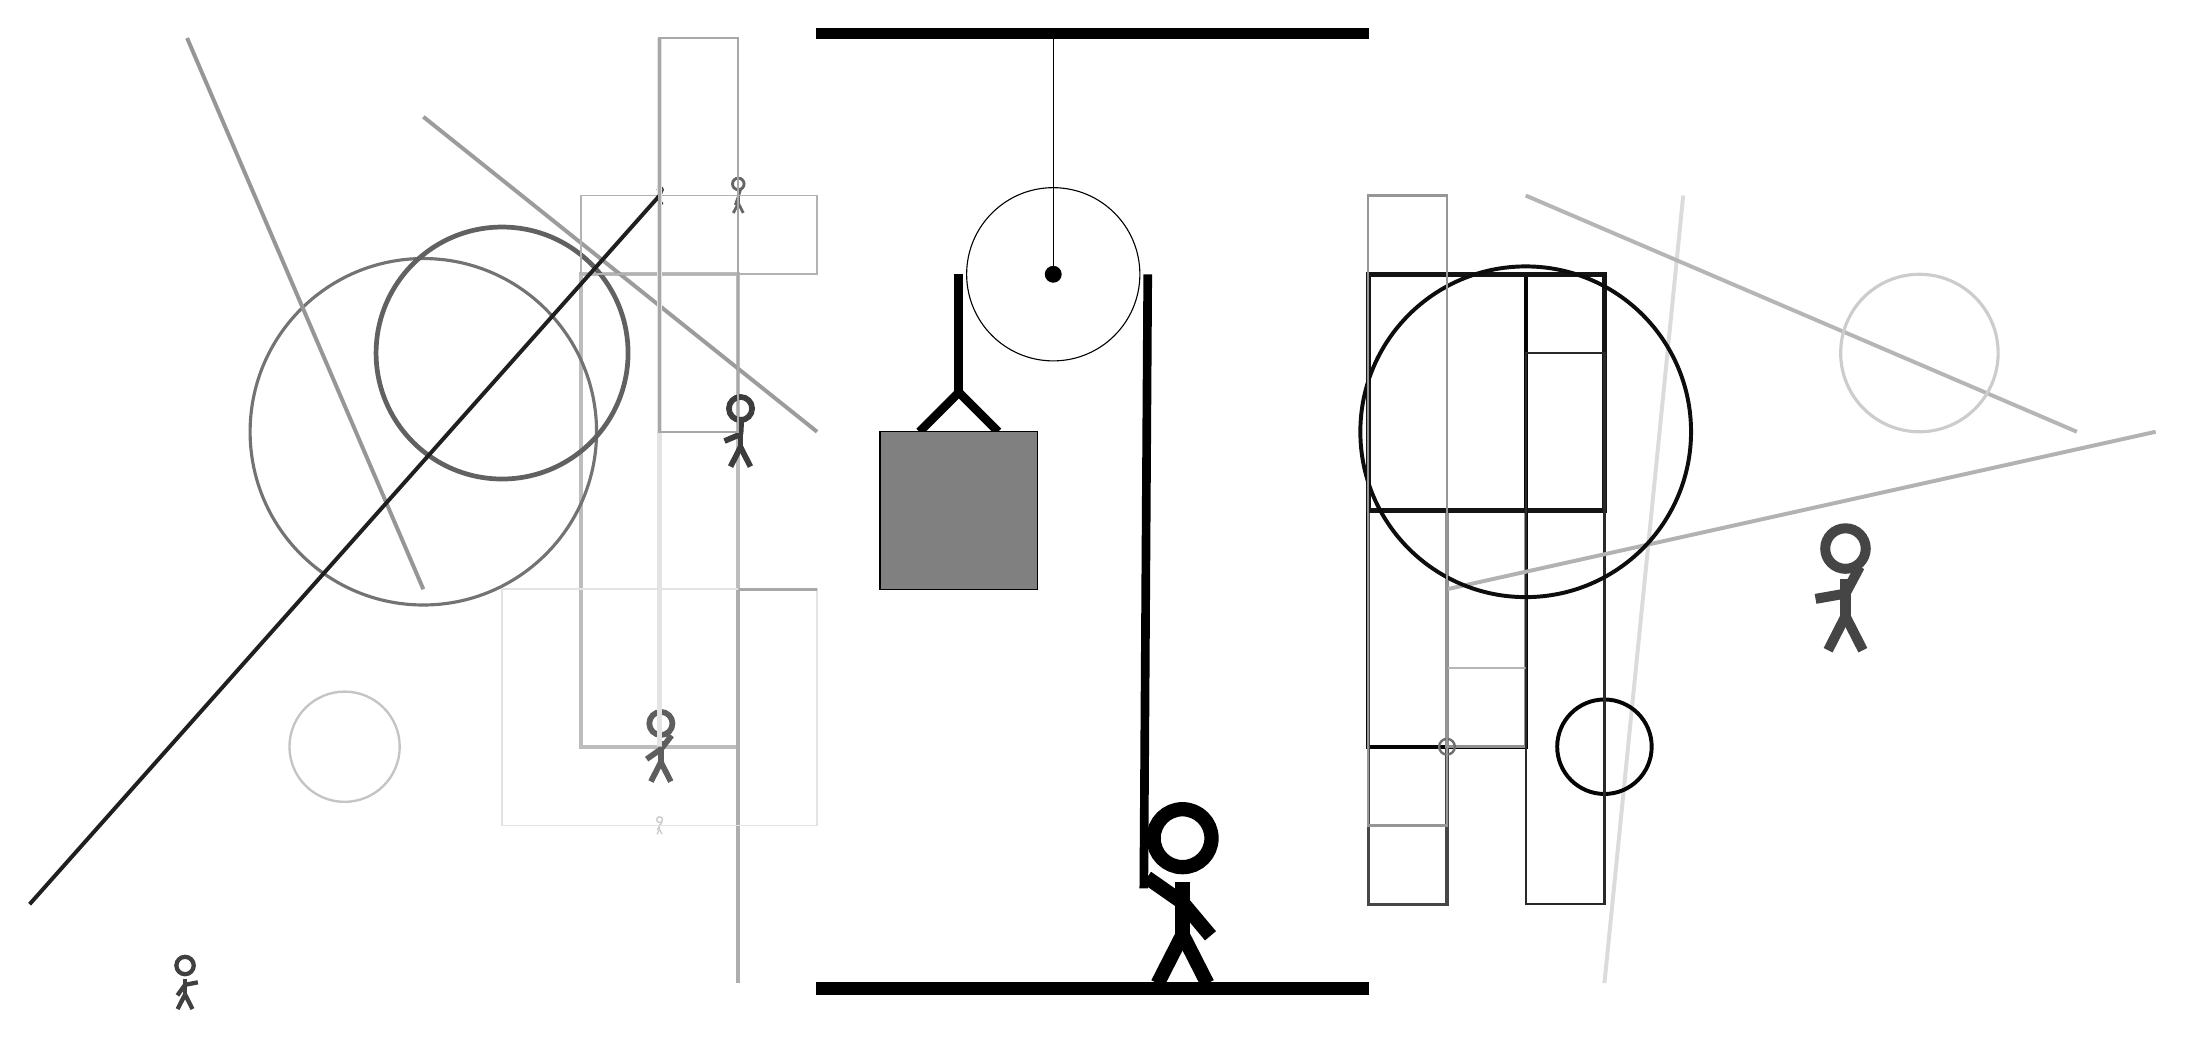
\begin{tikzpicture}
			%%%%% START %%%%%
			
			\draw[fill=black] (-2, 9) rectangle (5, 9.125);
			
			\draw (1, 6) circle (1.1);
			\draw[fill=black] (1, 6) circle (0.1);
			\draw (1, 9) -- (1, 6);
			
			\draw[line width=1.1mm] (-0.7, 4.0) -- (-0.2, 4.5) -- (0.3, 4.0);
			\draw[fill=black!50] (-1.2, 4.0) rectangle (0.8, 2.0);
			
			\draw[line width=1.1mm] (-0.2, 6) -- (-0.2, 4.5);
			\centerarc[line width=1.1mm](1, 6)(0:180:1.2000000000000002);
			\draw[line width=1.1mm](2.2, 6) -- (2.15, -1.8);
			
			\draw[line width=0.5mm, color=black!14](9, 7) -- (8, -3);
			
			\draw[line width=0.5mm, color=black!98] (7, 6) rectangle (5, 0);
			\draw[line width=0.5mm, color=black!26] (-3, 0) rectangle (-5, 6);
			\draw[line width=0.4mm, color=black!72] (6, 3) rectangle (5, -2);
			\node[line width=0.7mm, color=black!74] at (-4, 7) {\Strichmaxerl[1][0][63]};
			\draw[line width=0.4mm, color=black!43] (7, 3) rectangle (6, 0);
			
			\node[line width=0.2mm, color=black!20] at (-4, -1) {\Strichmaxerl[1][59][57]};
			\node[line width=0.6mm, color=black!60] at (-3, 7) {\Strichmaxerl[2][70][73]};
			\draw [line width=0.3mm, color=black!23](-8, 0) circle (0.7);
			
			\node[line width=0.2mm, color=black!63] at (-4, 0) {\Strichmaxerl[4][35][52]};
			
			\draw [line width=0.5mm, color=black!98](8, 0) circle (0.6);
			\node[line width=0.6mm, color=black!76] at (-3, 4) {\Strichmaxerl[4][23][87]};
			\draw[line width=0.6mm, color=black!92] (5, 3) rectangle (8, 6);
			
			\draw[line width=0.3mm, color=black!84] (7, -2) rectangle (8, 5);
			\draw [line width=0.4mm, color=black!55](-7, 4) circle (2.2);
			\draw[line width=0.5mm, color=black!30](6, 2) -- (15, 4);
			\draw[line width=0.3mm, color=black!29] (6, 1) rectangle (7, 1);
			
			\draw [line width=0.6mm, color=black!62](-6, 5) circle (1.6);
			\draw[line width=0.5mm, color=black!32] (-3, 2) rectangle (-3, -3);
			\draw[line width=0.5mm, color=black!39](-7, 8) -- (-2, 4);
			\draw[line width=0.5mm, color=black!41](-7, 2) -- (-10, 9);
			
			\node[line width=0.4mm, color=black!75] at (-10, -3) {\Strichmaxerl[3][54][11]};
			\draw[line width=0.2mm, color=black!30] (-2, 6) rectangle (-5, 7);
			\draw[line width=0.7mm, color=black!11] (-4, 9) rectangle (-4, 0);
			\draw[line width=0.5mm, color=black!29](7, 7) -- (14, 4);
			
			\draw[line width=0.2mm, color=black!11] (-2, -1) rectangle (-6, 2);
			\draw [line width=0.4mm, color=black!20](12, 5) circle (1.0);
			\draw [line width=0.3mm, color=black!57](6, 0) circle (0.1);
			\node[line width=0.5mm, color=black!73] at (11, 2) {\Strichmaxerl[7][10][62]};
			\draw[line width=0.4mm, color=black!34] (-2, 2) rectangle (-3, 2);
			\draw[line width=0.5mm, color=black!88](-4, 7) -- (-12, -2);
			
			\draw [line width=0.5mm, color=black!95](7, 4) circle (2.1);
			\draw[line width=0.3mm, color=black!41] (5, -1) rectangle (6, 7);
			\draw[line width=0.3mm, color=black!34] (-4, 9) rectangle (-3, 4);
			
			
			\node at (2.6, -1.9) {\Strichmaxerl[10][-35][-50]};
			
			\draw[fill=black] (-2, -3) rectangle (5, -3.15);
			
			%%%%% END %%%%%
		\end{tikzpicture}
	\end{figure}	
\end{document}